\documentclass[a4paper]{article}
\usepackage[utf8]{inputenc}
\usepackage[T1]{fontenc}
\usepackage[english]{babel}
\usepackage{fancyhdr}
\usepackage{lastpage}
\usepackage[left=2cm,right=2cm,top=2cm,bottom=4cm]{geometry}
\usepackage{scalerel}
\usepackage{enumerate}
\usepackage{xcolor}
\usepackage{listings}
\usepackage{xspace}
\usepackage{url}
\usepackage{lmodern}
\usepackage{float}

\definecolor{myblue}{rgb}{0.33,0.61,0.83}
\definecolor{mygreen}{rgb}{0.39,0.56,0.31}
\definecolor{myorange}{rgb}{0.80,0.56,0.47}

\lstset{
	basicstyle=\ttfamily,
	backgroundcolor=\color{gray!10!white},
    xleftmargin=6pt,
	framexleftmargin=6pt,
	xrightmargin=6pt,
    framexrightmargin=6pt,
    framextopmargin=6pt,
	framexbottommargin=6pt,
    frame=tb,
	framerule=0pt,
	columns=fullflexible,
	breaklines=true,
	tabsize=2,
	%commentstyle=\color{mygreen},
	%keywordstyle=\color{myblue},
	%stringstyle=\color{myorange}
}

\setlength{\headheight}{50pt}
\setlength\parindent{0pt}

\lhead{
\includegraphics[scale=0.8]{imgs/logo-mse.png} \vspace{8pt}}

\rhead{\textbf{Lab 1: Crawling, indexation and webpage search} \\ 
Romain Claret and Jonathan Rial \\ 
Web Mining}

\cfoot{Page \thepage\ / \pageref{LastPage}}

\pagestyle{fancy}

\begin{document}

\part*{Lab 1: Crawling, indexation and webpage search}
In this web mining laboratory, we will implement a crawler that visits a website and push the data to a Solr server. We will also create some fields for indexing interesting data. Then we will create a searcher in Java that query data from the Solr server. The architecture is represented below: \\

\begin{center}
	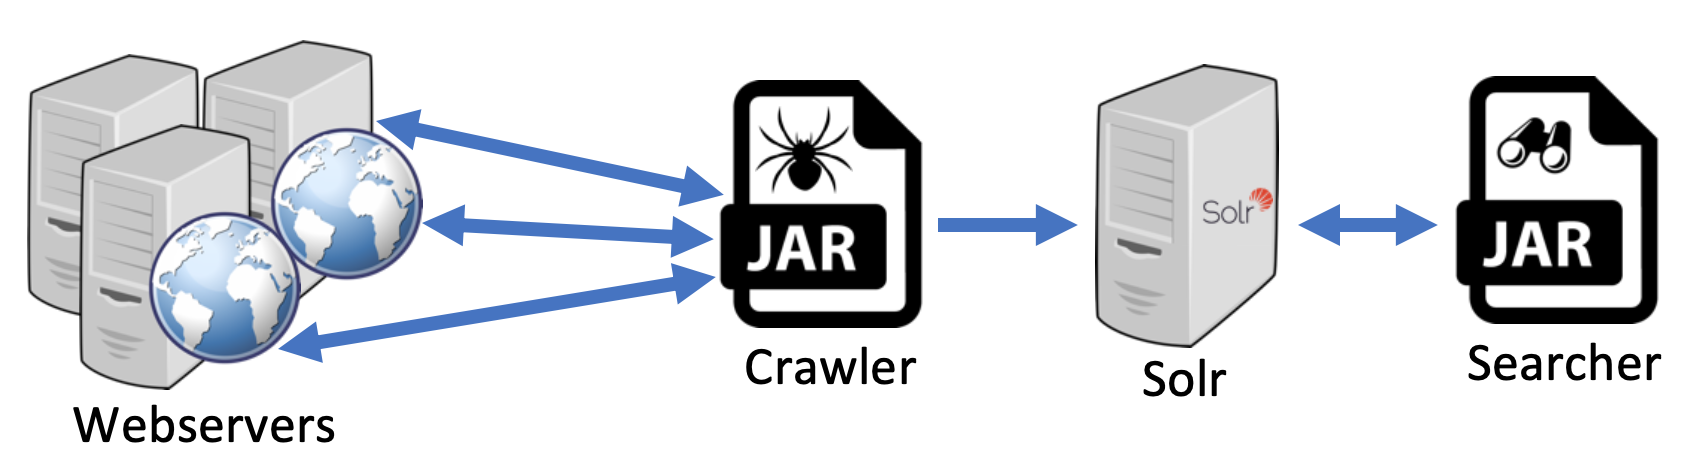
\includegraphics[scale=0.5]{imgs/architecture.png}
\end{center}

To implement the crawler, we used the library called Crawler4j and to parse the HTML we used Jsoup. These dependencies are automatically downloaded from Maven Central using Gradle. The following command runs our application: \\

\begin{lstlisting}[language=sh]
	$ gradle run
\end{lstlisting}

\vspace{6pt}

To simplify the installation, we used docker-solr as docker image for our Solr.

\section{Crawler}
\subsection{Core}
We started by creating a core for Solr, named \textit{core\_one} using the following command to attach to the docker bash:\\

\begin{lstlisting}[language=sh]
$ docker exec -u 0 -it docker-solr bash
\end{lstlisting}

then this command to create a default core.properties

\begin{lstlisting}[language=sh]
$ bin/solr create -c core_one
\end{lstlisting}

As we set \textit{update.autoCreateFields} to \textbf{false} in our core. We had to create two custom fields: \textit{doc\_title\_en} and \textit{doc\_body\_en}, which will be used to store the title and the body of each retained pages by the crawler.
\\
\subsection{Crawler4j}
We configured our crawler, \textbf{MyCrawler.java} to work with our Solr core \textit{core\_one}. Concerning our first crawler configuration:\\

\begin{itemize}  
\item starting page: wikipedia.org at "Veganism" page
\item domain limitation: yes
\item maximum pages to fetch: 70
\item maximum deepness: 2
\item politeness delay: 500
\item https: yes
\item FILTERS: custom binary files
\end{itemize}

\subsubsection{shouldVisit function}
We are applying the \textbf{FILTERS} pattern matching on the URL and verify that the domain.

\subsubsection{visit function}

The crawler retrieves the HTML page and parses them with jSoup. It creates a Solr document with the id field (hashcode of the page), the \textit{doc\_title\_en} (title from the page), and \textit{doc\_body\_en} (body content from the page) and finally adds the document into the current Solr instance.

To avoid Solr overloads, we set a loader for the commits. Indeed, the program will stock 50 documents before committing them to the Solr as a batch.

Each visited page has its content indexed by Solr.

\subsection{Tries and fails}
\begin{itemize}  
\item We first indexed \textbf{Vegan.com}, but the pages were not meaningful from a feature point of view, indeed it had no categories.
\end{itemize}

\section{Specific Indexation}
As a continuation of our work on the crawler, and a starting point for a more advanced specification, we duplicated our class \textbf{MyCrawler} into \textbf{MyCrawler2}. Indeed, the purpose here is to upgrade our crawler to gather more meaningful information.\\

In a will to make our indexation more performant, we increased the page limit to 2000 and removed the deepness limit.

We are parsing the following elements:
\begin{itemize}
\item en\_doc\_title: The title of the page (Fig. \ref{fig:title})
\item en\_doc\_body: The body of the page, its content
\item en\_doc\_categories: The categories of the page (Fig. \ref{fig:categories})
\item en\_doc\_topics: The topics of the page, the <h3> (Fig. \ref{fig:topics})
\item en\_doc\_infobox: The infobox of the page (Fig. \ref{fig:infobox})
\item en\_doc\_language: The language of the page
\item en\_doc\_navigations: The navigation of the page (Fig. \ref{fig:navigation})
\item en\_doc\_url: The URL of the page
\end{itemize}


\begin{figure}[H]
	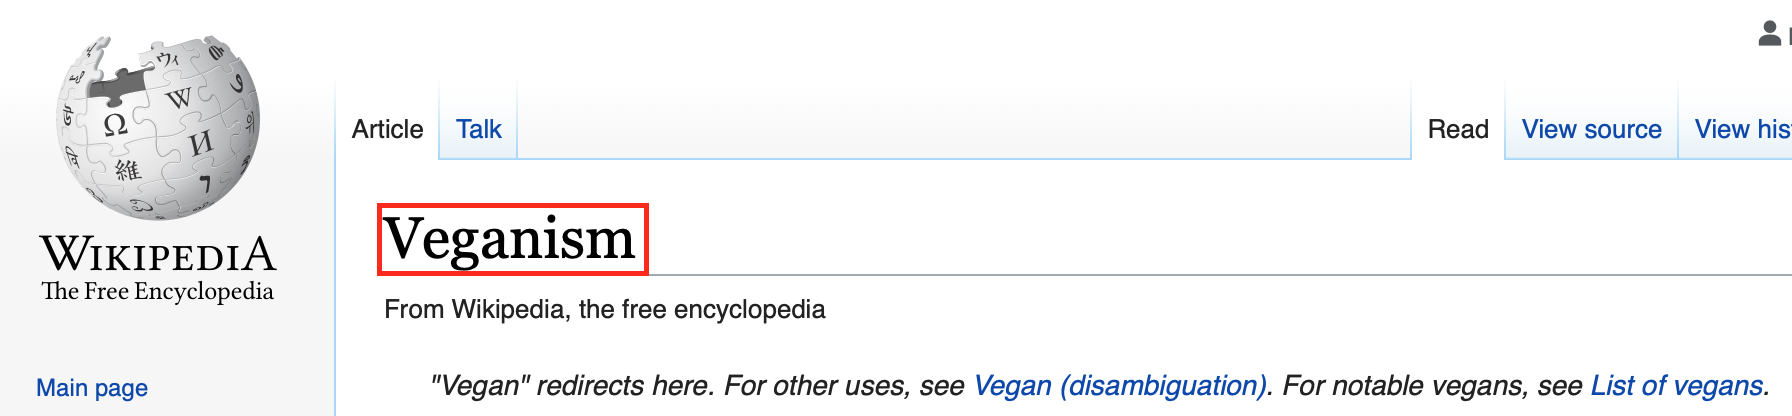
\includegraphics[width=\linewidth]{imgs/title}
	\caption{Wikipedia Title}
	\label{fig:title}
\end{figure}

\begin{figure}[H]
	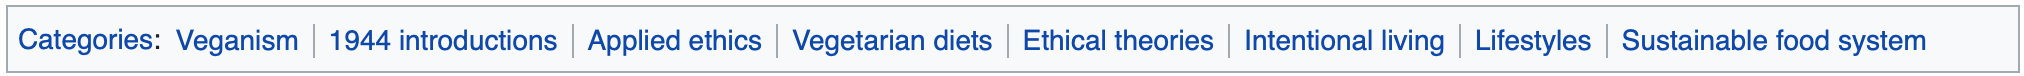
\includegraphics[scale=0.5]{imgs/categories}
	\caption{Wikipedia Categories}
	\label{fig:categories}
\end{figure}

\begin{figure}[H]
  \begin{minipage}[b]{0.4\textwidth}
    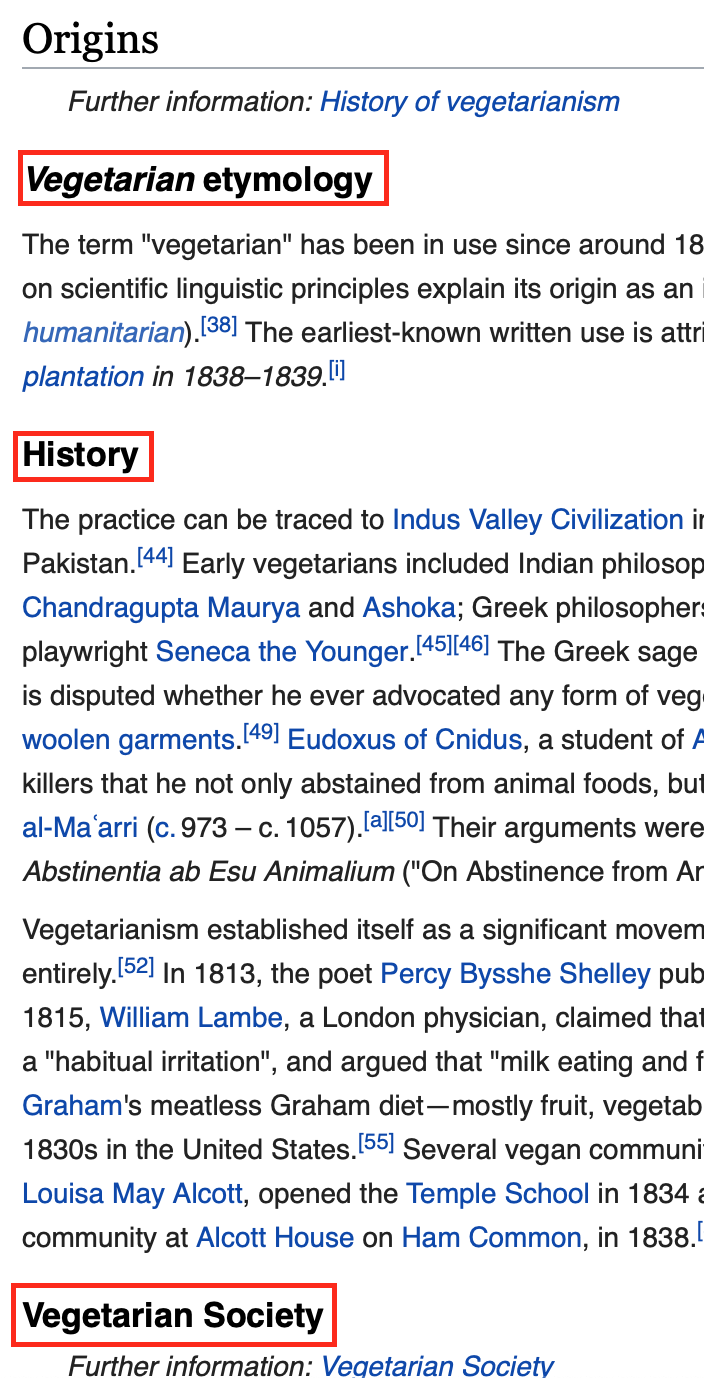
\includegraphics[width=\textwidth]{imgs/topics}
    \caption{Wikipedia Topics}
    \label{fig:topics}
  \end{minipage}
  \hfill
  \begin{minipage}[b]{0.4\textwidth}
    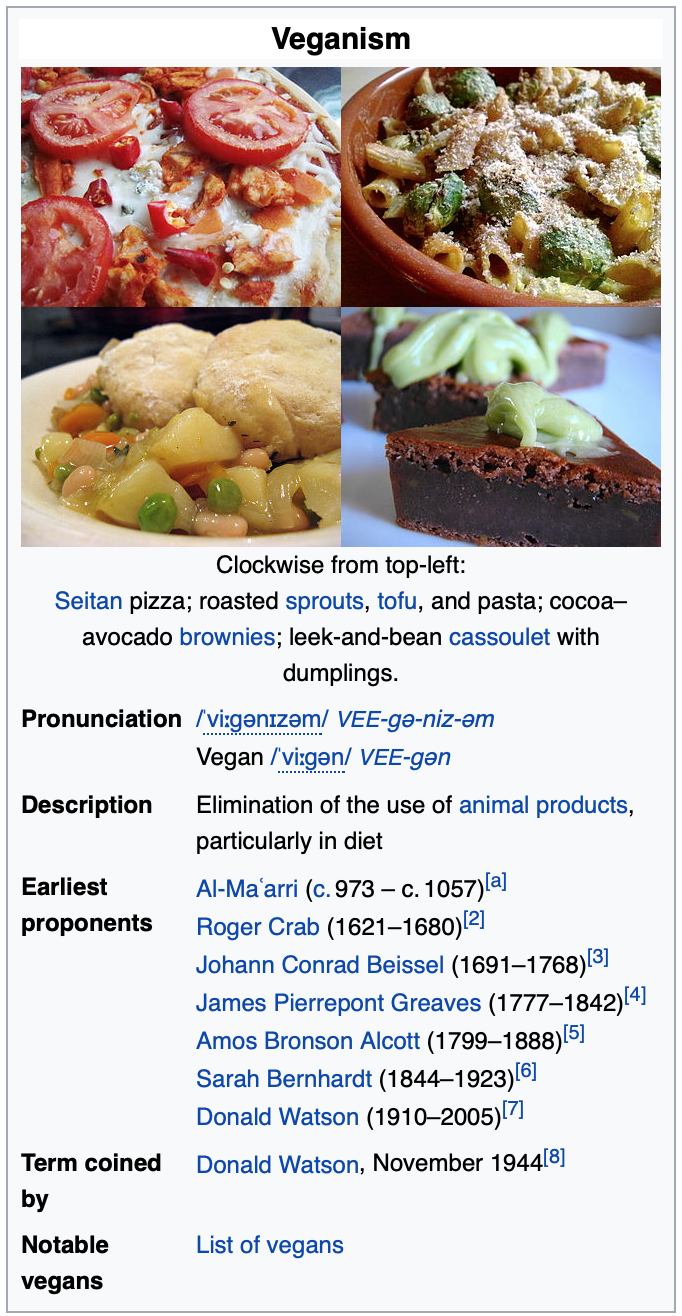
\includegraphics[width=\textwidth]{imgs/infobox}
    \caption{Wikipedia Infobox}
    \label{fig:infobox}
  \end{minipage}
\end{figure}

\begin{figure}[H]
	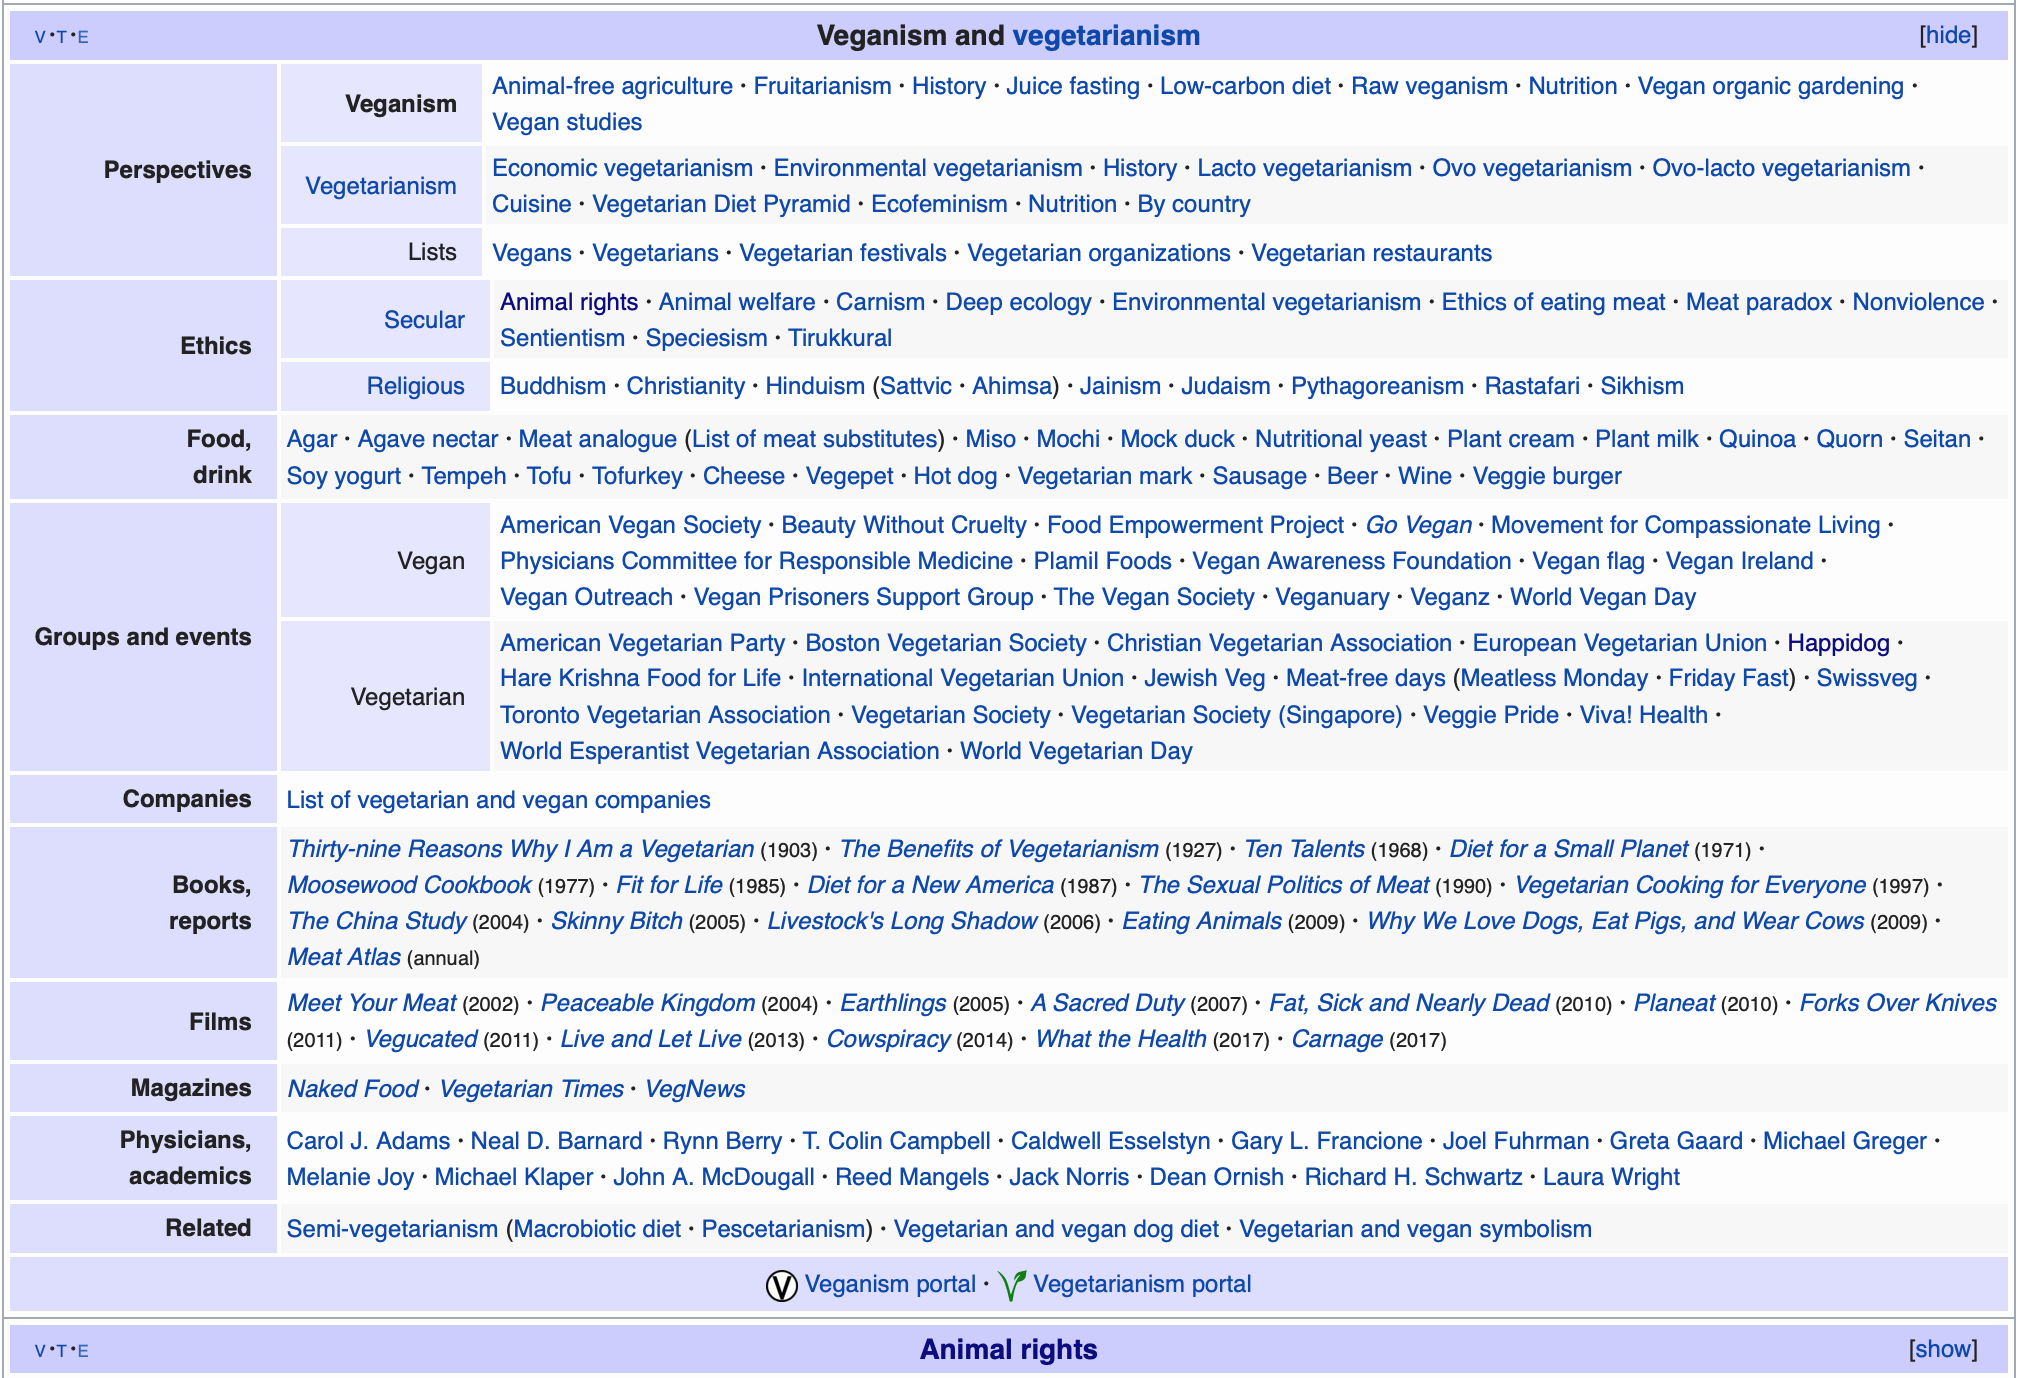
\includegraphics[scale=0.5]{imgs/navigation}
	\caption{Wikipedia Navigation}
	\label{fig:navigation}
\end{figure}

\section{Search}
Based on our MyCrawler2, we have asked to index up to 2000 webpages. Using the Solr web interface, we found out that 1995 documents were indeed indexed.\\

Continuing with Solr web interface, we can also search with a specific query such as Lactose into a specific field we extracted via our crawler. For example: en\_doc\_body:Lactose. \\

We implemented a searcher, Searcher.java, which also returns the score for each returned document. Moreover, we are using a weighting system on each extracted features. Indeed, the meaningfulness of each feature is not equivalent. \\

After some tweaking, we came out with the following formula, where <query> is the user's query :\\

q: (en\_doc\_title:<query>)\^{}6 (en\_doc\_topics:<query>)\^{}5 (en\_doc\_infobox:<query>)\^{}4\\
(en\_doc\_categories:<query>)\^{}3 (en\_doc\_navigations:<query>)\^{}2 (en\_doc\_body:<query>)\^{}1\\


We gave a weight of 6 for the title, a weight of 5 for the topics and so one. The lower is the weight; the lower is the importance is.\\

The following figures from 6 to 9 are query examples:

\begin{figure}[H]
  
  \begin{minipage}[b]{0.4\textwidth}
    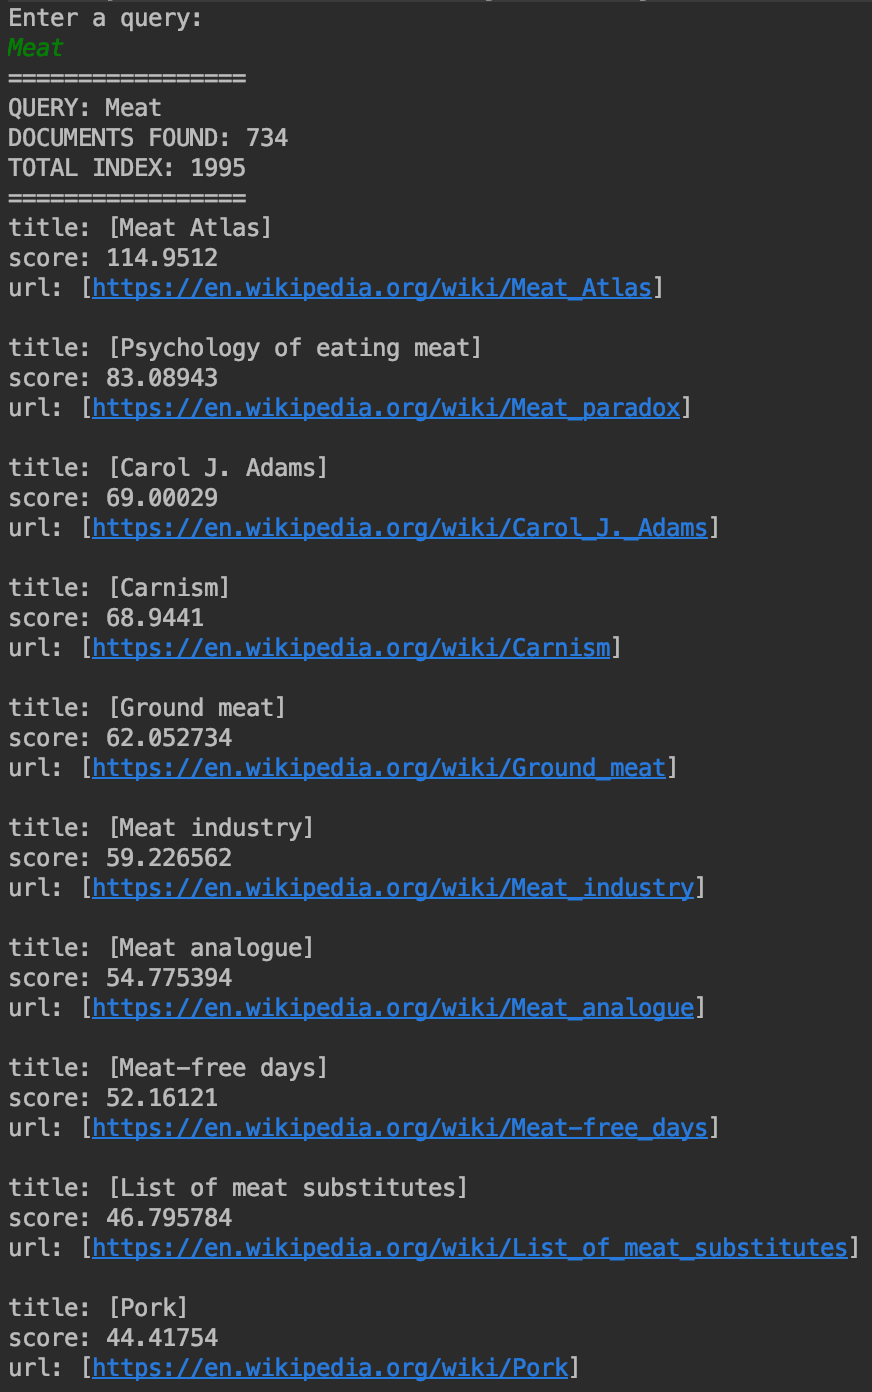
\includegraphics[width=\textwidth]{imgs/meat}
    \caption{Search Query: meat}
    \label{fig:meat}
  \end{minipage}
  \hfill
  \begin{minipage}[b]{0.4\textwidth}
    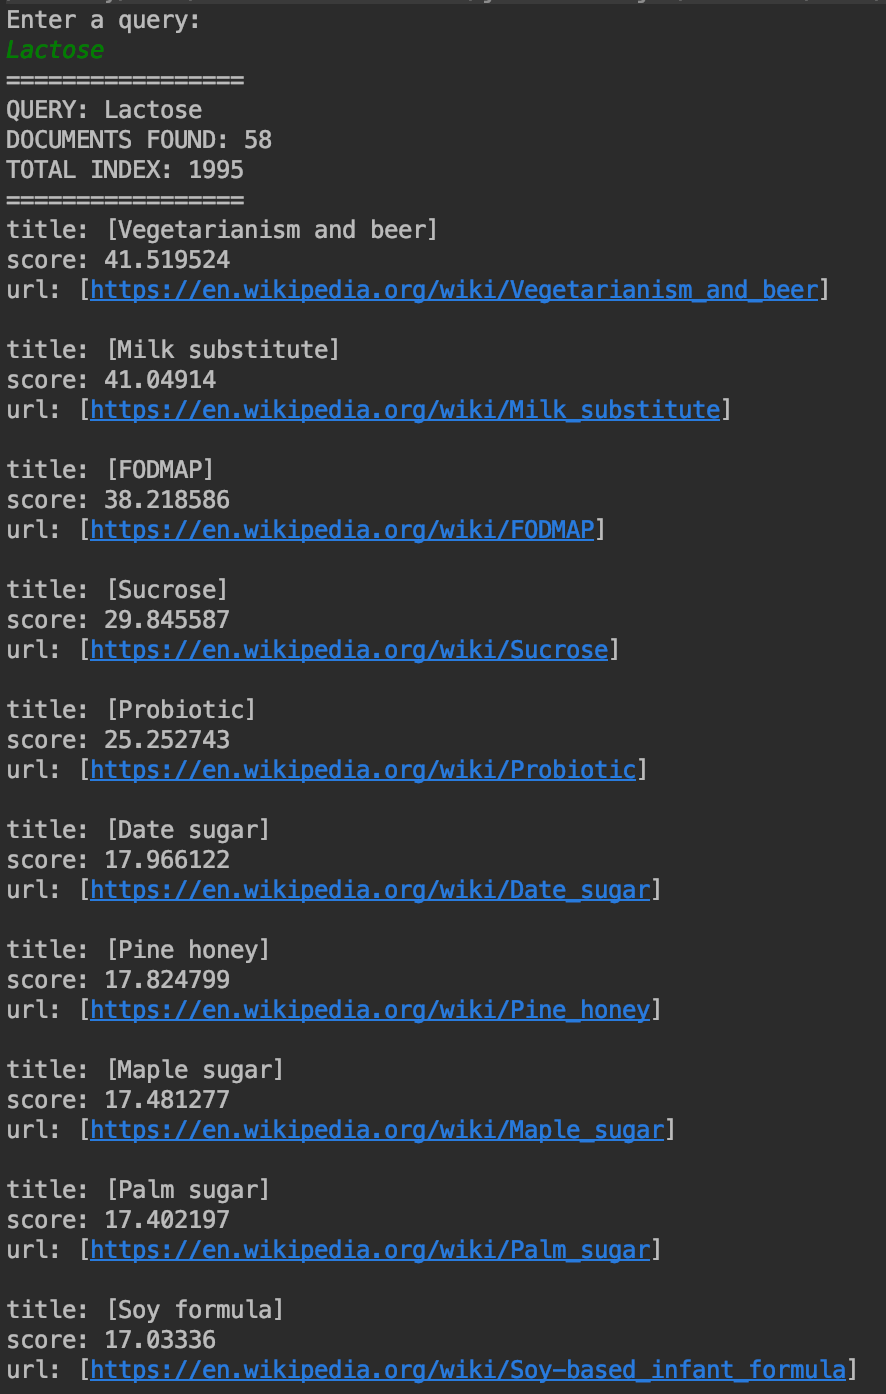
\includegraphics[width=\textwidth]{imgs/lactose}
    \caption{Search Query: lactose}
    \label{fig:lactose}
  \end{minipage}
  \\\\\\\\
  \begin{minipage}[b]{0.4\textwidth}
    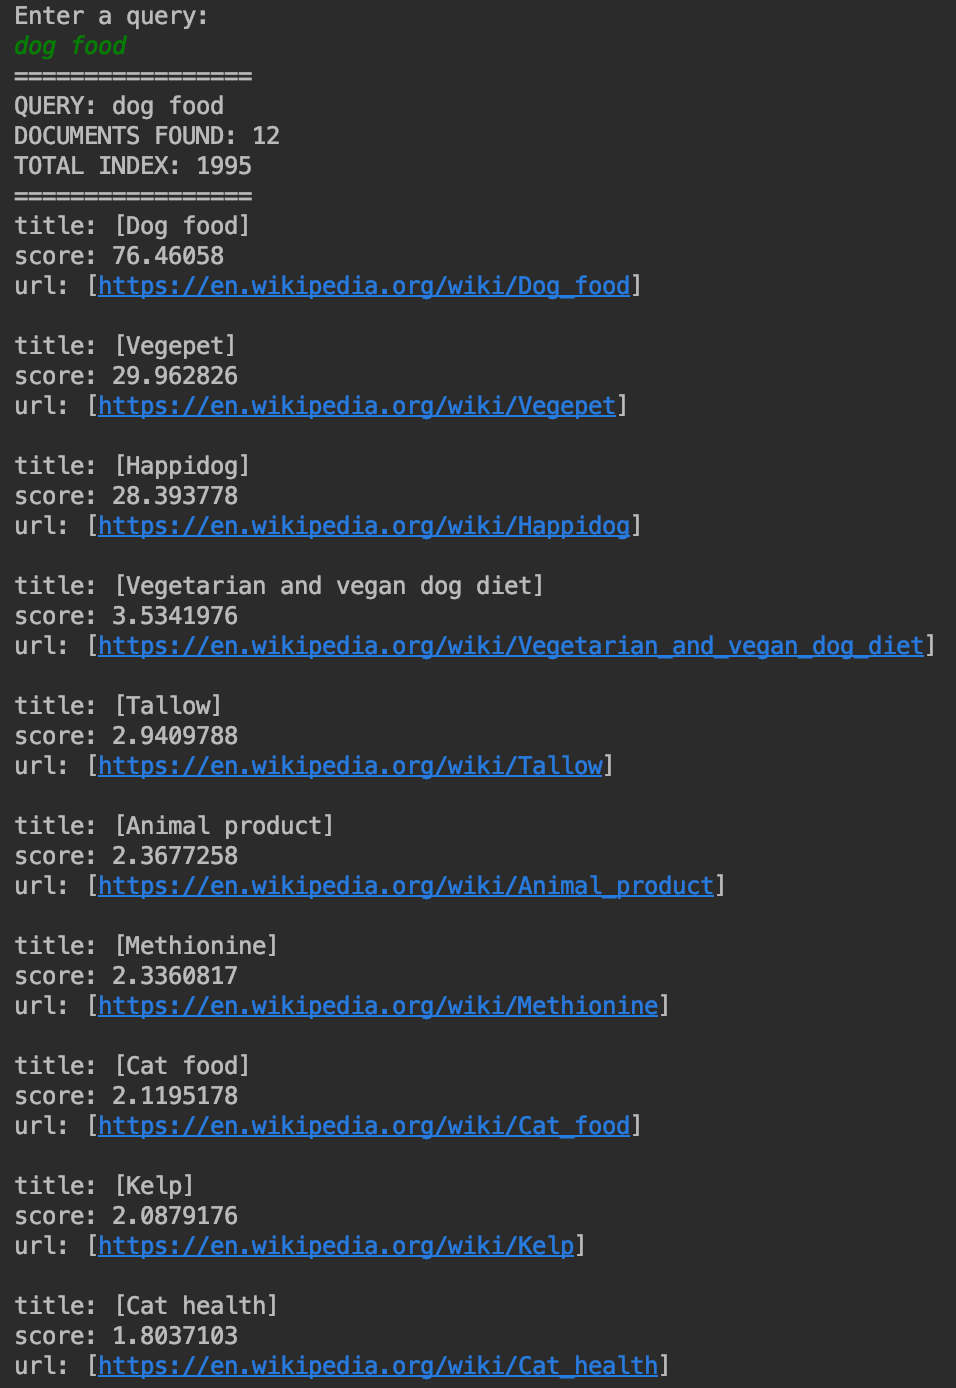
\includegraphics[width=\textwidth]{imgs/dog-food}
    \caption{Search Query: dog food}
    \label{fig:dog-food}
  \end{minipage}
  \hfill
  \begin{minipage}[b]{0.4\textwidth}
    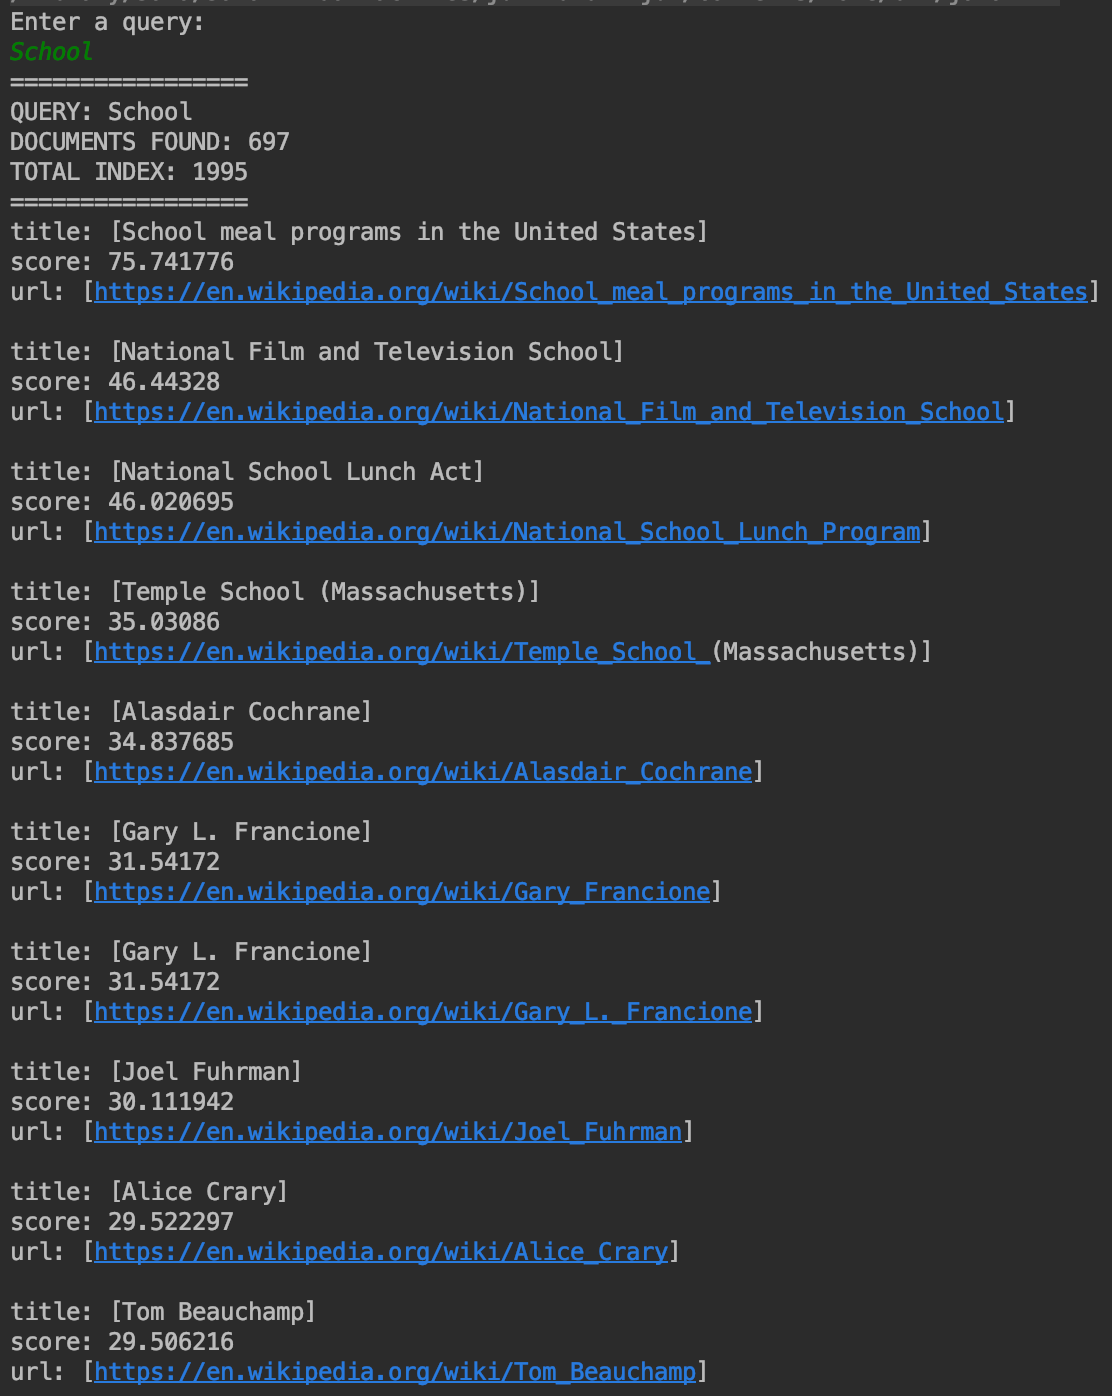
\includegraphics[width=\textwidth]{imgs/school}
    \caption{Search Query: School}
    \label{fig:school}
  \end{minipage}
\end{figure}



\section{Theorical questions}
\textbf{Please explain what strategy should be adopted for indexing pages in several languages (each page is composed of only one language, but the corpus includes pages in several languages). What should you watch out for? Please explain the process you propose.} \\

We could imagine different solutions to handle multiple languages with Solr:
\begin{itemize}  
    \item The first solution is to defined different schema fields for every language like "\texttt{title\_fr}" or "\texttt{title\_en}" and applying filters to each language. The downside of this solution is the high memory consumption and complexity when many languages are present.
    \item The second solution is to use a collection of same fields for all languages, add a field to store the langue and then apply a filter on it (e.g. \texttt{fq=language:english}). The downside of this solution is that we cannot use language specific features like lemmatization and stemming.
    \item The third solution is to create a Solr core for each language and route the queries to the right core.
    \item A fourth solution would be to index specific subdomains with specific tags or cores, such as en.wikipedia.org, fr.wikipedia.org, de.wikipedia.org, etc.
    \item In a fifth solution, we could try to modify Crawler's header by asking a specific language.
\end{itemize}
If we have a few languages to querying, we recommend to use the first solution, but if we have many languages, we recommend the third or fourth solution. \\

\textbf{Solr allows by default to do a fuzzy search. Please explain what it is and how Solr implements it. Some first names may have a lot of spelling variations (eg Caitlin : Caitilin, Caitlen, Caitlinn, Caitlyn, Caitlyne, Caitlynn, Cateline, Catelinn, Catelyn, Catelynn, Catlain, Catlin, Catline, Catlyn, Catlynn, Kaitlin, Kaitlinn, Kaitlyn, Kaitlynn, Katelin, Katelyn, Katelynn, etc). Is it possible to use, while keeping a good performance, the fuzzy search made available by Solr to do search taking into account such variations? If not what alternative(s) do you see, please justify your answer.} \\

The fuzzy search matches a term when the edit distance between the query and the document's term is under an arbitrary threshold. According to the JavaDoc, this threshold is by default at $2$. \\

Yes, it is possible to use the fuzzy search and keeping good performance. Solr is based on Lucene, and from version 4, its library uses a Levenshtein Automaton, a deterministic automaton (DFA) that accepts only the terms within edit distance $N$. It is possible to compute this automaton of degree $N$ for an input word $W$ time linear in the length of $W$. \\

Concerning the Caitlin example, by using the \textbf{\~} operator, we can specify a distance, for exemple \textit{aitlin \~{} 2}. If it's still not enough, we can combine the fuzzy search with the \textbf{OR} operator: \textit{aitlin \~{} 2 OR Kaitlynn \~{} 2}.

However, in most of the cases, stemming gives similar results to the fuzzy search, and we could also mention the lemmatization.\\

For more informations: \url{http://citeseerx.ist.psu.edu/viewdoc/summary?doi=10.1.1.16.652}

\subsection{Conclusion}

We learned a lot on the principle of webpage crawling with the help of this laboratory. Indeed, it was nice to see how Solr builds an index based on the crawled, and how it is possible to tweak the extracted features to make the indexation even better.\\

Finally, we were pleasantly surprised about how well the search based on the Solr indexation work, we didn't expect to have such meaningful matchings.

\end{document}

